\documentclass[11pt,a4paper]{article}
%%%%%%%%%%%%%%%%%%%%%%%%% Credit %%%%%%%%%%%%%%%%%%%%%%%%

% template ini dibuat oleh martin.manullang@if.itera.ac.id untuk dipergunakan oleh seluruh sivitas akademik itera.

%%%%%%%%%%%%%%%%%%%%%%%%% PACKAGE starts HERE %%%%%%%%%%%%%%%%%%%%%%%%
\usepackage{graphicx}
\usepackage{caption}
\usepackage{microtype}
\captionsetup[table]{name=Tabel}
\captionsetup[figure]{name=Gambar}
\usepackage{tabulary}
\usepackage{minted}
\usepackage{amsmath}
\usepackage{fancyhdr}
\usepackage{amssymb}
\usepackage{amsthm}
\usepackage{float}
\usepackage{enumitem}
\usepackage{multicol}
\usepackage{placeins}
\usepackage{amsfonts}
\usepackage{graphicx}
\usepackage{fancyvrb}
\usepackage[all]{xy}
\usepackage{tikz}
\usepackage{verbatim}
\usepackage[left=2cm,right=2cm,top=3cm,bottom=2.5cm]{geometry}
\usepackage{hyperref}
\hypersetup{
    colorlinks,
    linkcolor={red!50!black},
    citecolor={blue!50!black},
    urlcolor={blue!80!black}
}
\usepackage{caption}
\usepackage{subcaption}
\usepackage{multirow}
\usepackage{psfrag}
\usepackage[T1]{fontenc}
\usepackage[scaled]{beramono}
% Enable inserting code into the document
\usepackage{listings}
\usepackage{xcolor} 
% custom color & style for listing
\definecolor{codegreen}{rgb}{0,0.6,0}
\definecolor{codegray}{rgb}{0.5,0.5,0.5}
\definecolor{codepurple}{rgb}{0.58,0,0.82}
\definecolor{backcolour}{rgb}{0.95,0.95,0.92}
\definecolor{LightGray}{gray}{0.9}
\lstdefinestyle{mystyle}{
	backgroundcolor=\color{backcolour},   
	commentstyle=\color{green},
	keywordstyle=\color{codegreen},
	numberstyle=\tiny\color{codegray},
	stringstyle=\color{codepurple},
	basicstyle=\ttfamily\footnotesize,
	breakatwhitespace=false,         
	breaklines=true,                 
	captionpos=b,                    
	keepspaces=true,                 
	numbers=left,                    
	numbersep=5pt,                  
	showspaces=false,                
	showstringspaces=false,
	showtabs=false,                  
	tabsize=2
}
\lstset{style=mystyle}
\renewcommand{\lstlistingname}{Kode}
%%%%%%%%%%%%%%%%%%%%%%%%% PACKAGE ends HERE %%%%%%%%%%%%%%%%%%%%%%%%


%%%%%%%%%%%%%%%%%%%%%%%%% Data Diri %%%%%%%%%%%%%%%%%%%%%%%%
\newcommand{\student}{\textbf{Fathan Andi Kartagama (122140055)}}
\newcommand{\course}{\textbf{Sistem Teknologi Multimedia (IF25-40305)}}
\newcommand{\assignment}{\textbf{Worksheet 1: Setup Python Environment untuk Multimedia}}

%%%%%%%%%%%%%%%%%%% using theorem style %%%%%%%%%%%%%%%%%%%%
\newtheorem{thm}{Theorem}
\newtheorem{lem}[thm]{Lemma}
\newtheorem{defn}[thm]{Definition}
\newtheorem{exa}[thm]{Example}
\newtheorem{rem}[thm]{Remark}
\newtheorem{coro}[thm]{Corollary}
\newtheorem{quest}{Question}[section]
%%%%%%%%%%%%%%%%%%%%%%%%%%%%%%%%%%%%%%%%
\usepackage{lipsum}%% a garbage package you don't need except to create examples.
\usepackage{fancyhdr}
\pagestyle{fancy}
\lhead{Fathan Andi Kartagama (122140055)}
\rhead{ \thepage}
\cfoot{\textbf{Worksheet 1: Setup Python Environment untuk Multimedia}}
\renewcommand{\headrulewidth}{0.4pt}
\renewcommand{\footrulewidth}{0.4pt}

%%%%%%%%%%%%%%  Shortcut for usual set of numbers  %%%%%%%%%%%

\newcommand{\N}{\mathbb{N}}
\newcommand{\Z}{\mathbb{Z}}
\newcommand{\Q}{\mathbb{Q}}
\newcommand{\R}{\mathbb{R}}
\newcommand{\C}{\mathbb{C}}
\setlength\headheight{14pt}

%%%%%%%%%%%%%%%%%%%%%%%%%%%%%%%%%%%%%%%%%%%%%%%%%%%%%%%555
\begin{document}
\thispagestyle{empty}
\begin{center}
	
\includegraphics[scale = 0.15]{Figure/ifitera-header.png}
	\vspace{0.1cm}
\end{center}
\noindent
\rule{17cm}{0.2cm}\\[0.3cm]
Nama: \student \hfill Tugas Ke: \assignment\\[0.1cm]
Mata Kuliah: \course \hfill Tanggal: \today\\
\rule{17cm}{0.05cm}
\vspace{0.1cm}



%%%%%%%%%%%%%%%%%%%%%%%%%%%%%%%%%%%%%%%%%%%%% BODY DOCUMENT %%%%%%%%%%%%%%%%%%%%%%%%%%%%%%%%%%%%%%%%%%%%%
\section{Instruksi Tugas}

\subsection{Persiapan}
\begin{itemize}
    \item Menginstall Python 3.8 atau lebih baru (disarankan 3.10)
    \item Memilih salah satu tool manajemen environment: \textbf{conda}, \textbf{venv}, atau \textbf{uv}. Pada mata kuliah ini saya menggunakan manajemen environtment \href{https://docs.astral.sh/uv/}{UV}
    \item Membuka terminal/command prompt
    \item Menyiapkan dokumen \LaTeX\ ini untuk dokumentasi
\end{itemize}

\subsection{Bagian 1: Membuat Environment Python}
\subsubsection{Menggunakan uv}
\begin{lstlisting}[language=bash, caption=Membuat environment dengan uv]
# Install uv terlebih dahulu jika belum ada
pip install uv

# bisa dengan powershell (Windows)
powershell -ExecutionPolicy ByPass -c "irm https://astral.sh/uv/install.ps1 | iex"

# atau terminal (MacOS dan Linux)
curl -LsSf https://astral.sh/uv/install.sh | sh

# Membuat environment baru
uv venv multimedia-uv

# Mengaktifkan environment (Linux/Mac)
source multimedia-uv/bin/activate

# Mengaktifkan environment (Windows)
multimedia-uv\Scripts\activate

# Verifikasi environment aktif (MacOS dan Linux)
which python

# Verifikasi environtment aktif (Windows)
## Jika Menggunakan CMD
where python

## Jika Menggunakan Powershell
Get-Command python | Select-Object -ExpandProperty Source

\end{lstlisting}

\textbf{Dokumentasikan di sini:}
\begin{itemize}
    \item Tool manajemen environment yang Anda pilih: \textbf{[UV]}
    \item Screenshot atau copy-paste output dari perintah verifikasi environment
    \begin{figure}[h!]
    \centering
    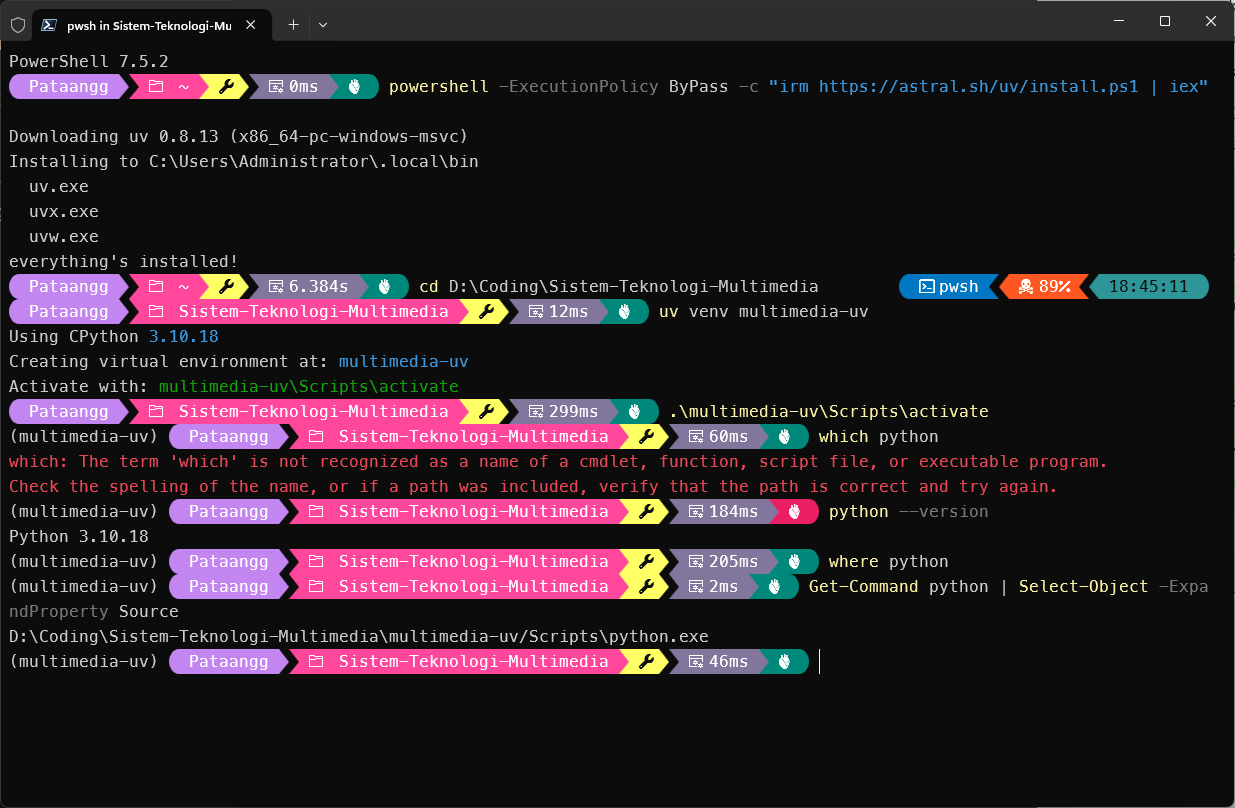
\includegraphics[scale = 0.5]{Figure/img1.png}
    \caption{Output verifikasi environment}
    \vspace{0.1cm}
    \end{figure}
\end{itemize}

\subsection{Bagian 2: Instalasi Library Multimedia}
Setelah environment aktif, install library-library berikut:

\subsubsection{Library Audio Processing}
\begin{lstlisting}[language=bash, caption=Instalasi library audio]
# Untuk pip (venv/uv):
pip install librosa soundfile scipy
\end{lstlisting}

\subsubsection{Library Image Processing}
\begin{lstlisting}[language=bash, caption=Instalasi library image]
# Untuk pip (venv/uv):
pip install opencv-python pillow scikit-image matplotlib
\end{lstlisting}

\subsubsection{Library Video Processing}
\begin{lstlisting}[language=bash, caption=Instalasi library video]
# Untuk pip (venv/uv):
pip install moviepy imageio-ffmpeg
\end{lstlisting}

\subsubsection{Library General Purpose}
\begin{lstlisting}[language=bash, caption=Instalasi library umum]
# Untuk pip (venv/uv):
pip install numpy pandas jupyter
\end{lstlisting}

\textbf{Dokumentasikan di sini:}
\begin{itemize}[leftmargin=*]
  \item Perintah instalasi yang Anda gunakan:
    \begin{itemize}
      \item Audio: \verb|uv pip install librosa soundfile scipy|
      \item Image: \verb|uv pip install opencv-python pillow scikit-image matplotlib|
      \item Video: \verb|uv pip install moviepy imageio-ffmpeg|
      \item General: \verb|uv pip install numpy pandas jupyter|
    \end{itemize}

  \item Screenshot proses instalasi atau output sukses:
    \begin{figure}[h]
      \centering

      \begin{subfigure}[b]{0.48\textwidth}
        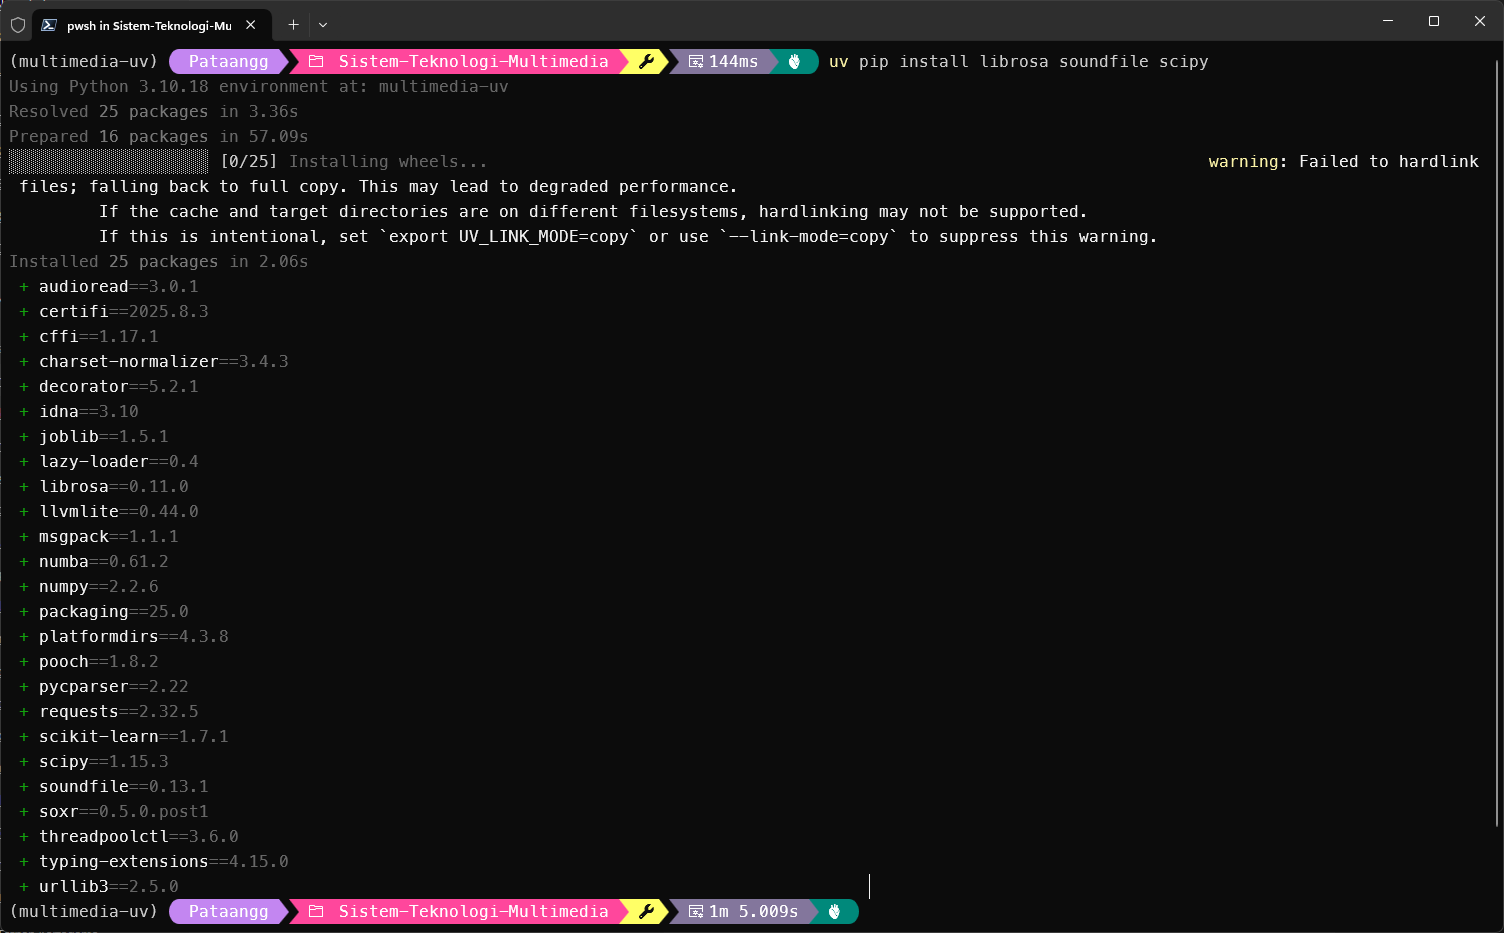
\includegraphics[width=\linewidth]{Figure/img2.png}
        \caption{Audio}
      \end{subfigure}\hfill
      \begin{subfigure}[b]{0.48\textwidth}
        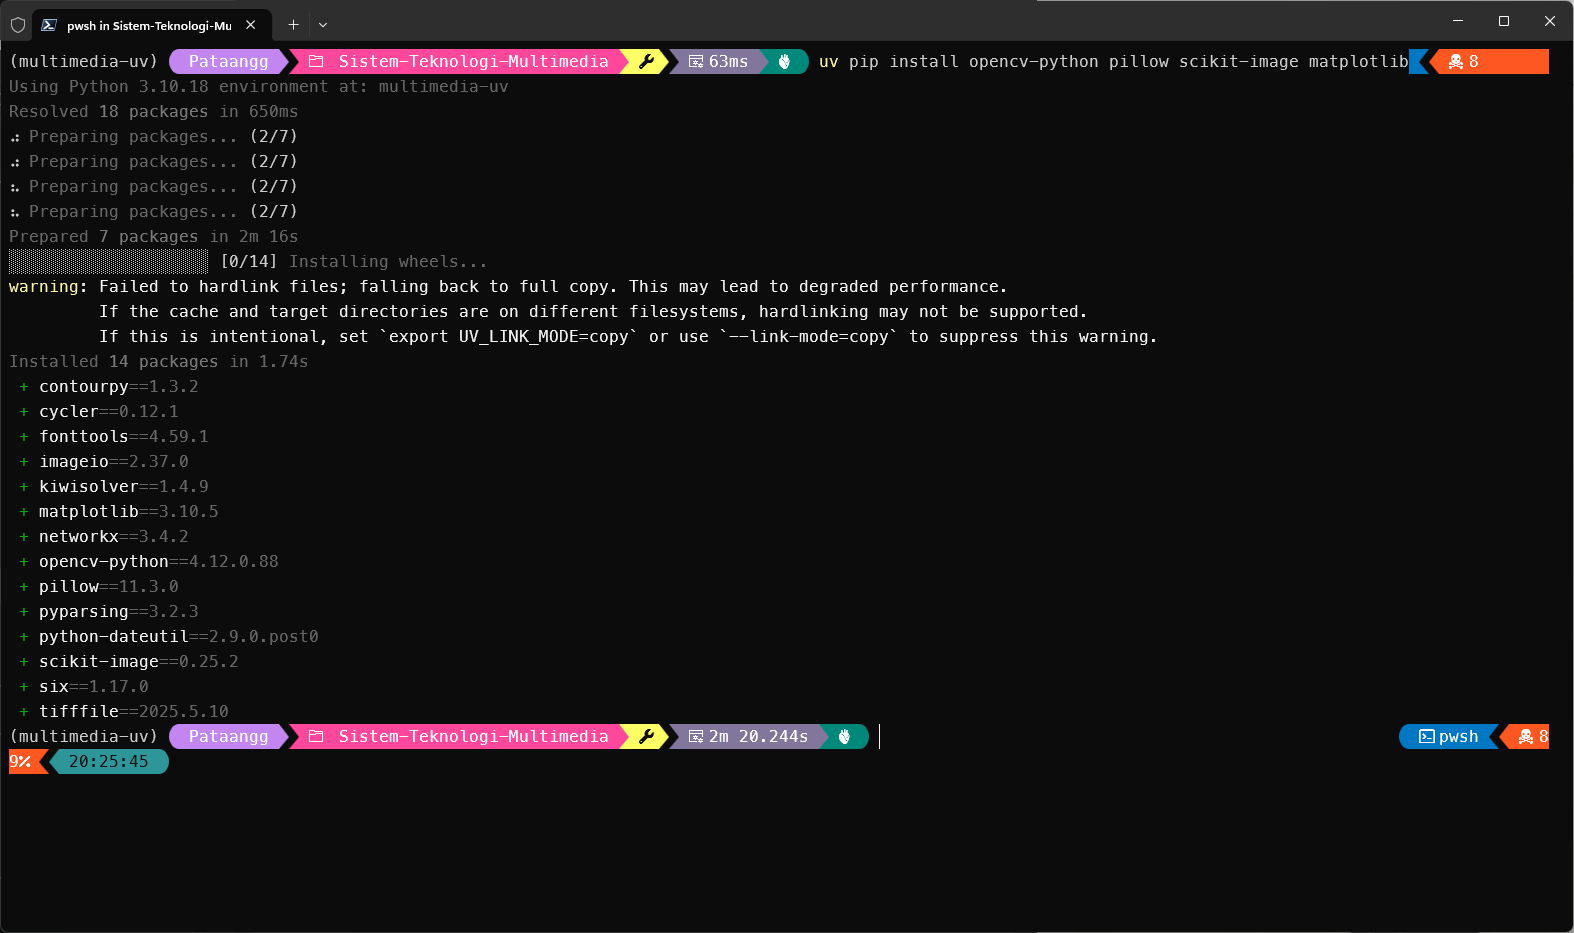
\includegraphics[width=\linewidth]{Figure/img3.png}
        \caption{Image}
      \end{subfigure}

      \vspace{0.5em}

      \begin{subfigure}[b]{0.48\textwidth}
        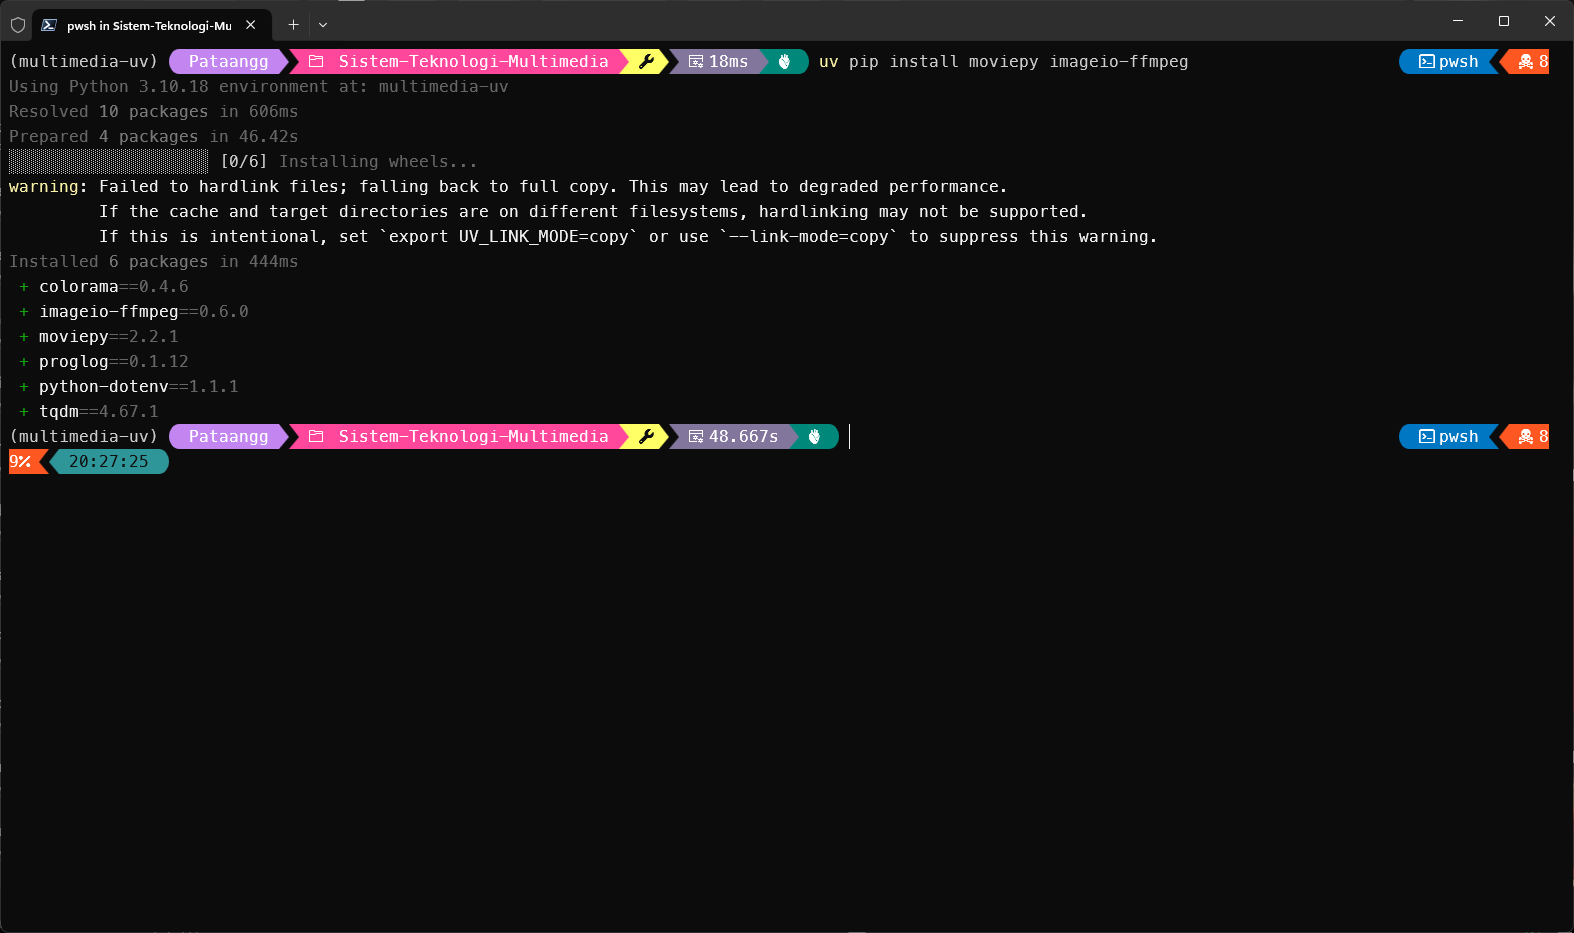
\includegraphics[width=\linewidth]{Figure/img4.png} % <-- fixed extension
        \caption{Video}
      \end{subfigure}\hfill
      \begin{subfigure}[b]{0.48\textwidth}
        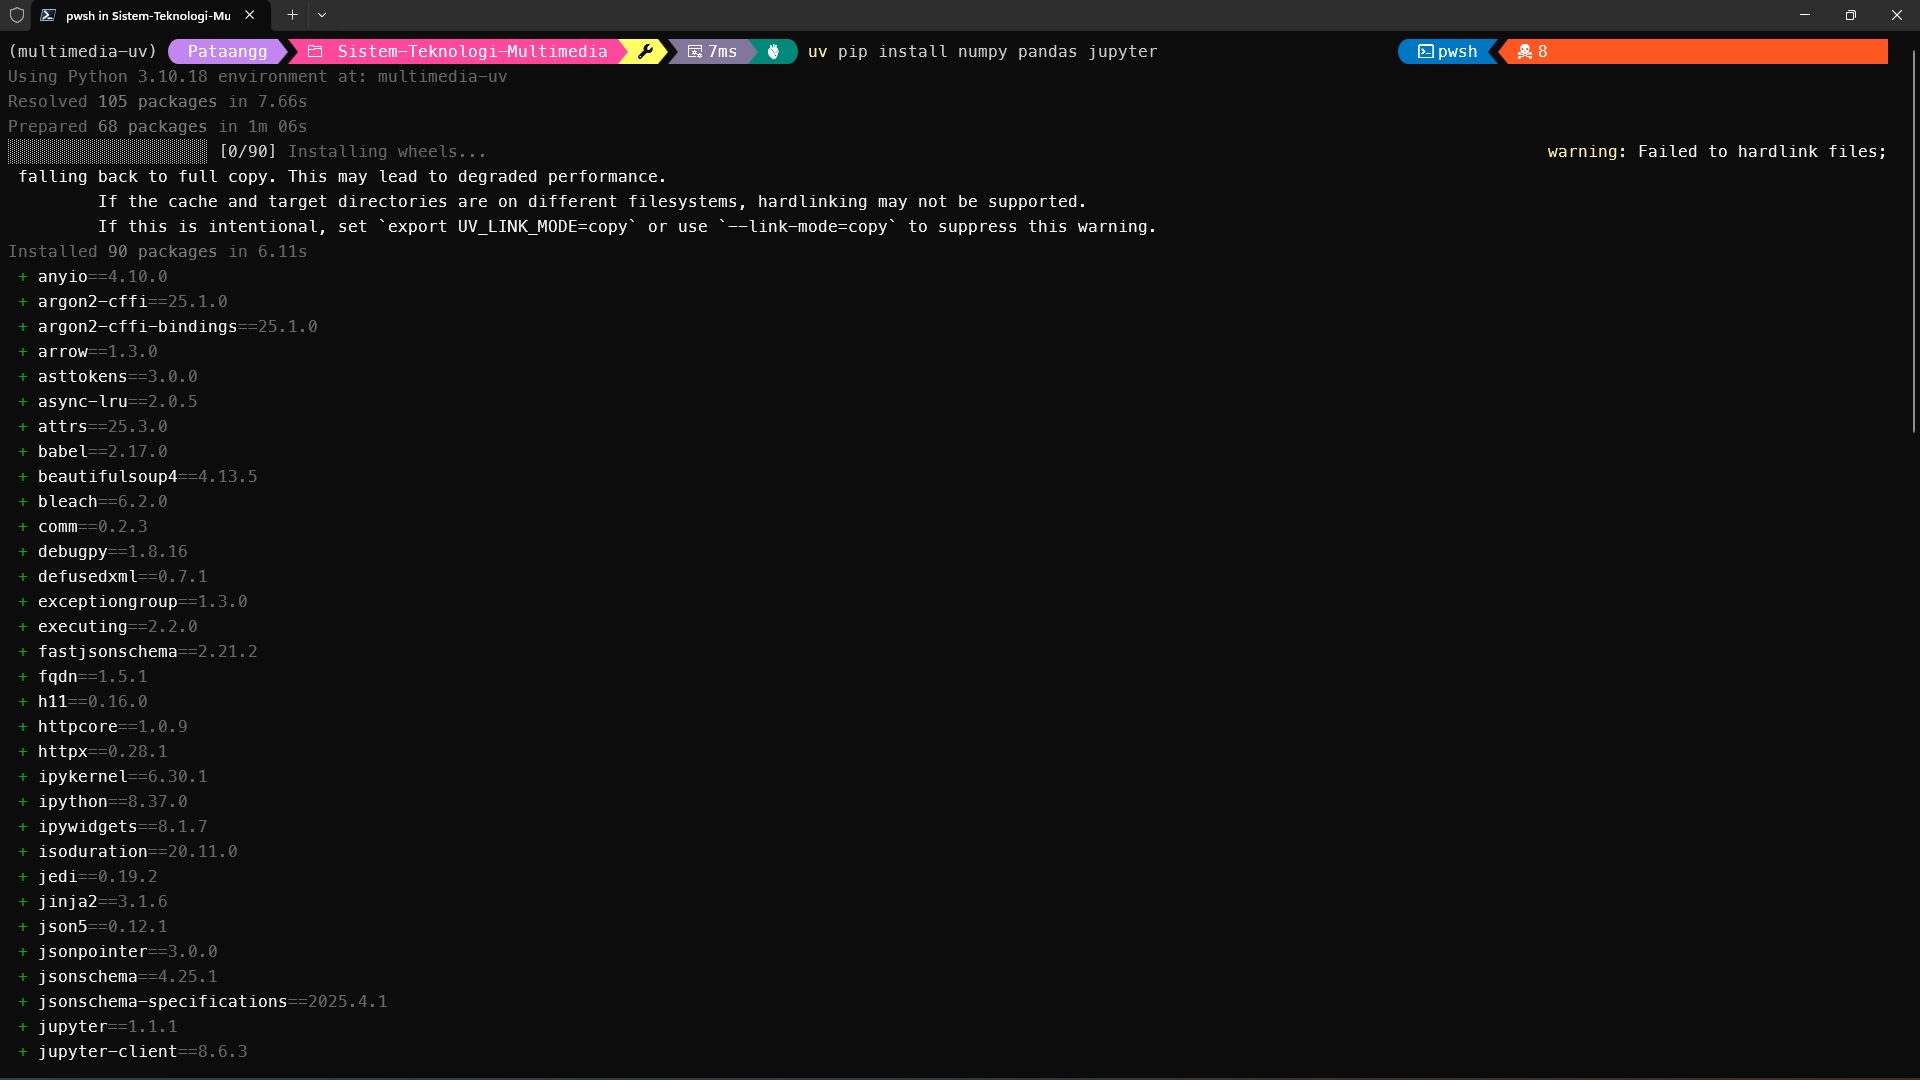
\includegraphics[width=\linewidth]{Figure/img5.png}
        \caption{General}
      \end{subfigure}

      \caption{Screenshots of installation steps in \texttt{uv} environment}
      \label{fig:uv-install-steps}
    \end{figure}
\end{itemize}

\begin{itemize}[leftmargin=*]
  \item Daftar library yang berhasil diinstall dengan versinya:

  {\scriptsize
  \begin{multicols}{3}
  \begin{Verbatim}
anyio==4.10.0
argon2-cffi==25.1.0
argon2-cffi-bindings==25.1.0
arrow==1.3.0
asttokens==3.0.0
async-lru==2.0.5
attrs==25.3.0
audioread==3.0.1
babel==2.17.0
beautifulsoup4==4.13.5
bleach==6.2.0
certifi==2025.8.3
cffi==1.17.1
charset-normalizer==3.4.3
colorama==0.4.6
comm==0.2.3
contourpy==1.3.2
cycler==0.12.1
debugpy==1.8.16
decorator==5.2.1
defusedxml==0.7.1
exceptiongroup==1.3.0
executing==2.2.0
fastjsonschema==2.21.2
fonttools==4.59.1
fqdn==1.5.1
h11==0.16.0
httpcore==1.0.9
httpx==0.28.1
idna==3.10
imageio==2.37.0
imageio-ffmpeg==0.6.0
ipykernel==6.30.1
ipython==8.37.0
ipywidgets==8.1.7
isoduration==20.11.0
jedi==0.19.2
jinja2==3.1.6
joblib==1.5.1
json5==0.12.1
jsonpointer==3.0.0
jsonschema==4.25.1
jsonschema-specifications==2025.4.1
jupyter==1.1.1
jupyter-client==8.6.3
jupyter-console==6.6.3
jupyter-core==5.8.1
jupyter-events==0.12.0
jupyter-lsp==2.2.6
jupyter-server==2.17.0
jupyter-server-terminals==0.5.3
jupyterlab==4.4.6
jupyterlab-pygments==0.3.0
jupyterlab-server==2.27.3
jupyterlab-widgets==3.0.15
kiwisolver==1.4.9
lark==1.2.2
lazy-loader==0.4
librosa==0.11.0
llvmlite==0.44.0
markupsafe==3.0.2
matplotlib==3.10.5
matplotlib-inline==0.1.7
mistune==3.1.3
moviepy==2.2.1
msgpack==1.1.1
nbclient==0.10.2
nbconvert==7.16.6
nbformat==5.10.4
nest-asyncio==1.6.0
networkx==3.4.2
notebook==7.4.5
notebook-shim==0.2.4
numba==0.61.2
numpy==2.2.6
opencv-python==4.12.0.88
overrides==7.7.0
packaging==25.0
pandas==2.3.2
pandocfilters==1.5.1
parso==0.8.5
pillow==11.3.0
platformdirs==4.3.8
pooch==1.8.2
proglog==0.1.12
prometheus-client==0.22.1
prompt-toolkit==3.0.51
psutil==7.0.0
pure-eval==0.2.3
pycparser==2.22
pygments==2.19.2
pyparsing==3.2.3
python-dateutil==2.9.0.post0
python-dotenv==1.1.1
python-json-logger==3.3.0
pytz==2025.2
pywin32==311
pywinpty==3.0.0
pyyaml==6.0.2
pyzmq==27.0.2
referencing==0.36.2
requests==2.32.5
rfc3339-validator==0.1.4
rfc3986-validator==0.1.1
rfc3987-syntax==1.1.0
rpds-py==0.27.0
scikit-image==0.25.2
scikit-learn==1.7.1
scipy==1.15.3
send2trash==1.8.3
setuptools==80.9.0
six==1.17.0
sniffio==1.3.1
soundfile==0.13.1
soupsieve==2.7
soxr==0.5.0.post1
stack-data==0.6.3
terminado==0.18.1
threadpoolctl==3.6.0
tifffile==2025.5.10
tinycss2==1.4.0
tomli==2.2.1
tornado==6.5.2
tqdm==4.67.1
traitlets==5.14.3
types-python-dateutil==2.9.0.20250822
typing-extensions==4.15.0
tzdata==2025.2
uri-template==1.3.0
urllib3==2.5.0
wcwidth==0.2.13
webcolors==24.11.1
webencodings==0.5.1
websocket-client==1.8.0
widgetsnbextension==4.0.14
  \end{Verbatim}
  \end{multicols}
  }
\end{itemize}



\subsection{Bagian 3: Verifikasi Instalasi}
Buat file Python sederhana untuk menguji semua library yang telah diinstall:
\begin{lstlisting}[language=python, caption=Kode Python Sederhana untuk Cek library terinstall]
import importlib

# Daftar library dari requirements.txt
libraries = [
    "anyio", "argon2", "arrow", "asttokens", "async_lru", "attrs", "audioread",
    "babel", "bs4", "bleach", "certifi", "cffi", "charset_normalizer", "colorama",
    "comm", "contourpy", "cycler", "debugpy", "decorator", "defusedxml", "exceptiongroup",
    "executing", "fastjsonschema", "fonttools", "fqdn", "h11", "httpcore", "httpx",
    "idna", "imageio", "imageio_ffmpeg", "ipykernel", "IPython", "ipywidgets",
    "isoduration", "jedi", "jinja2", "joblib", "json5", "jsonpointer", "jsonschema",
    "jupyter", "jupyter_client", "jupyter_console", "jupyter_core", "jupyter_events",
    "jupyter_lsp", "jupyter_server", "jupyter_server_terminals", "jupyterlab",
    "jupyterlab_pygments", "jupyterlab_server", "jupyterlab_widgets", "kiwisolver",
    "lark", "lazy_loader", "librosa", "llvmlite", "markupsafe", "matplotlib",
    "matplotlib_inline", "mistune", "moviepy", "msgpack", "nbclient", "nbconvert",
    "nbformat", "nest_asyncio", "networkx", "notebook", "notebook_shim", "numba",
    "numpy", "cv2", "overrides", "packaging", "pandas", "pandocfilters", "parso",
    "PIL", "platformdirs", "pooch", "proglog", "prometheus_client", "prompt_toolkit",
    "psutil", "pure_eval", "pycparser", "pygments", "pyparsing", "dateutil",
    "dotenv", "python_json_logger", "pytz", "pywin32", "pywinpty", "yaml", "zmq",
    "referencing", "requests", "rfc3339_validator", "rfc3986_validator",
    "rfc3987_syntax", "rpds", "skimage", "sklearn", "scipy", "send2trash",
    "setuptools", "six", "sniffio", "soundfile", "soupsieve", "soxr", "stack_data",
    "terminado", "threadpoolctl", "tifffile", "tinycss2", "tomli", "tornado",
    "tqdm", "traitlets", "types_python_dateutil", "typing_extensions", "tzdata",
    "uri_template", "urllib3", "wcwidth", "webcolors", "webencodings",
    "websocket", "widgetsnbextension"
]

failed = []

print("🔍 Testing installed libraries...\n")

for lib in libraries:
    try:
        importlib.import_module(lib)
        print(f"✅ {lib} imported successfully")
    except Exception as e:
        print(f"❌ {lib} failed -> {e}")
        failed.append(lib)

print("\n=== SUMMARY ===")
if not failed:
    print("🎉 All libraries imported successfully!")
else:
    print(f"⚠️ Failed to import {len(failed)} libraries: {failed}")

\end{lstlisting}
\textbf{Jalankan script dan dokumentasikan hasilnya:}
\begin{figure}[H]
    \centering
    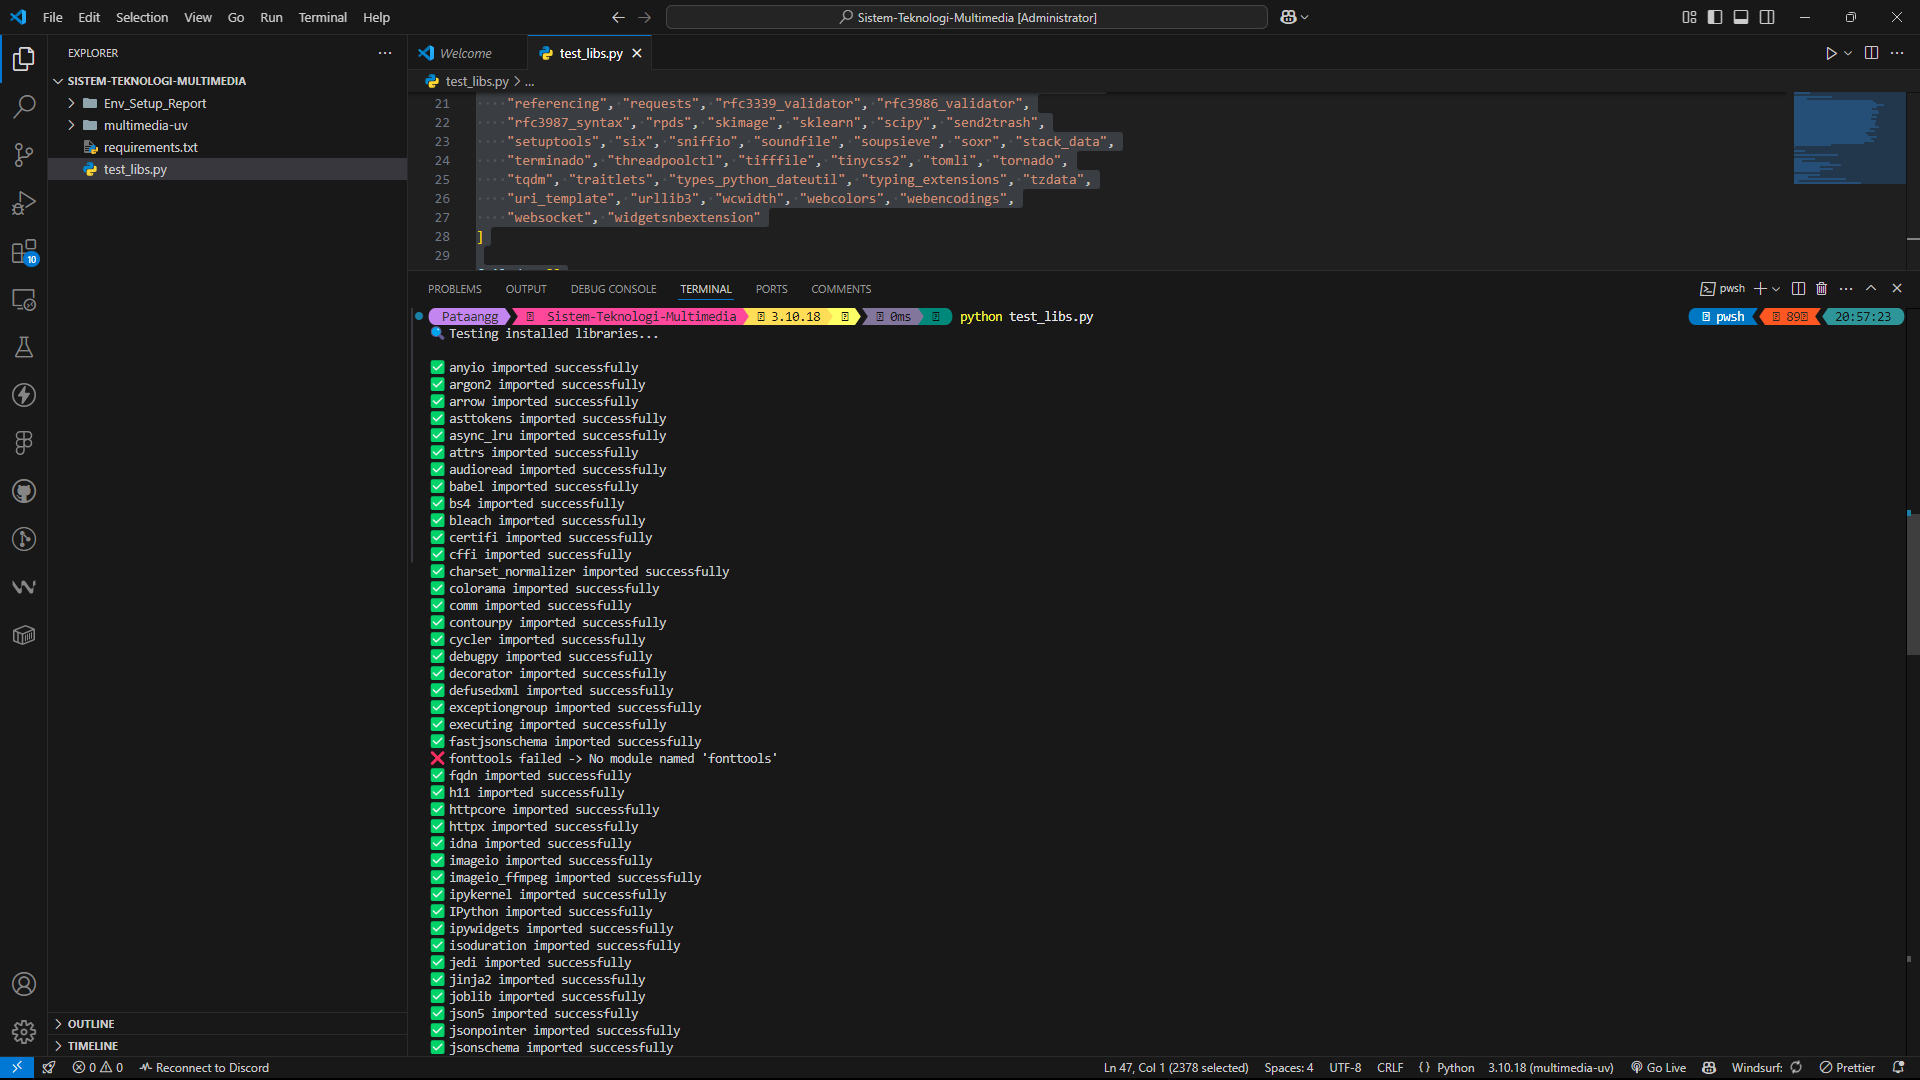
\includegraphics[scale = 0.25]{Figure/img6.png}
    \caption{Script Python sederhana untuk cek library}
    \vspace{0.1cm}
    
\end{figure}

\subsection{Bagian 4: Simple Test dengan Sample Code}
Buat dan jalankan contoh sederhana untuk setiap kategori multimedia:

\subsubsection{Test Audio Processing}
\begin{lstlisting}[language=Python, caption=Test audio processing sederhana]
import numpy as np
import matplotlib.pyplot as plt

# Generate simple sine wave
duration = 2  # seconds
sample_rate = 44100
frequency = 440  # A4 note

t = np.linspace(0, duration, int(sample_rate * duration))
audio_signal = np.sin(2 * np.pi * frequency * t)

# Plot waveform
plt.figure(figsize=(10, 4))
plt.plot(t[:1000], audio_signal[:1000])  # Plot first 1000 samples
plt.title('Sine Wave (440 Hz)')
plt.xlabel('Time (s)')
plt.ylabel('Amplitude')
plt.grid(True)
plt.savefig('sine_wave_test.png', dpi=150, bbox_inches='tight')
plt.show()

print(f"Generated {duration}s sine wave at {frequency}Hz")
print(f"Sample rate: {sample_rate}Hz")
print(f"Total samples: {len(audio_signal)}")
\end{lstlisting}

\subsubsection{Test Image Processing}
\begin{lstlisting}[language=Python, caption=Test image processing sederhana]
import numpy as np
import matplotlib.pyplot as plt
from PIL import Image

# Create a simple test image
width, height = 400, 300
image = np.zeros((height, width, 3), dtype=np.uint8)

# Add some patterns
image[:, :width//3, 0] = 255  # Red section
image[:, width//3:2*width//3, 1] = 255  # Green section
image[:, 2*width//3:, 2] = 255  # Blue section

# Add a white circle in the center
center_x, center_y = width//2, height//2
radius = 50
Y, X = np.ogrid[:height, :width]
mask = (X - center_x)**2 + (Y - center_y)**2 <= radius**2
image[mask] = [255, 255, 255]

# Display and save
plt.figure(figsize=(8, 6))
plt.imshow(image)
plt.title('Test Image with RGB Stripes and White Circle')
plt.axis('off')
plt.savefig('test_image.png', dpi=150, bbox_inches='tight')
plt.show()

print(f"Created test image: {width}x{height} pixels")
print(f"Image shape: {image.shape}")
print(f"Image dtype: {image.dtype}")
\end{lstlisting}

\textbf{Dokumentasikan hasil eksekusi:}
\begin{itemize}
    \item Screenshot output dari kedua script di atas
    \begin{figure}[h]
        \centering
        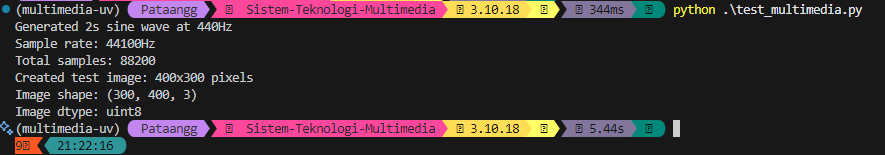
\includegraphics[width=0.8\textwidth]{Figure/img7.png}
        \caption{Screenshot output terminal dari kedua script}
        \vspace{0.1cm}
    \end{figure}
    \begin{figure}[H]
    \centering
    \begin{subfigure}[b]{0.48\textwidth}
        \centering
        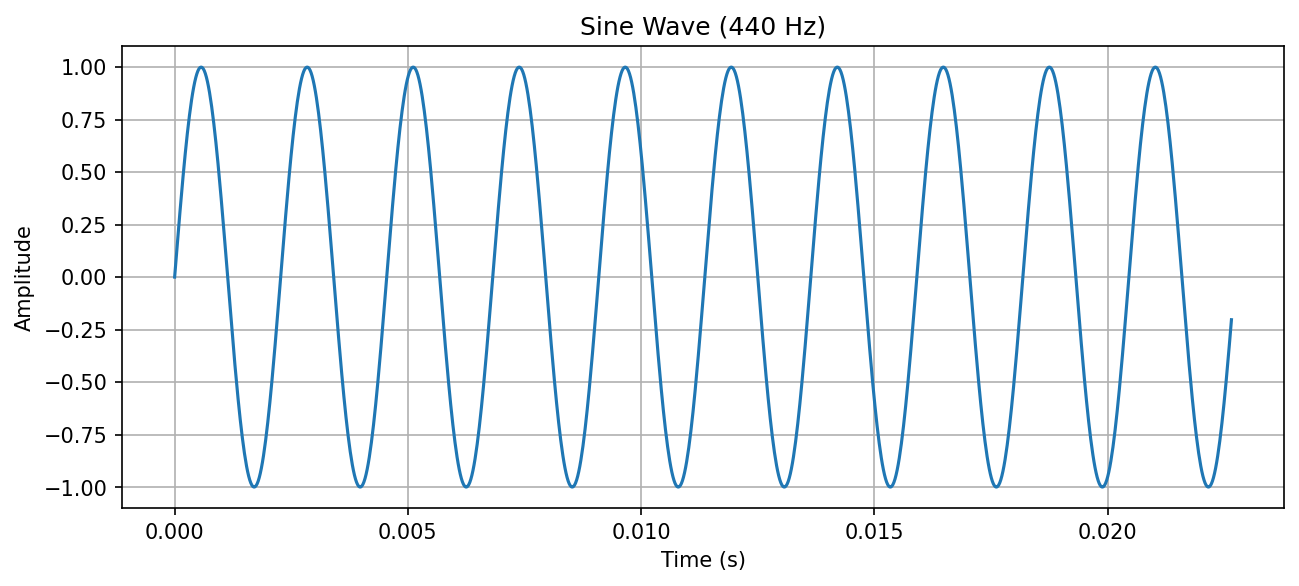
\includegraphics[width=\linewidth]{Figure/sine_wave_test.png}
        \caption{Sine Wave}
    \end{subfigure}\hfill
    \begin{subfigure}[b]{0.48\textwidth}
        \centering
        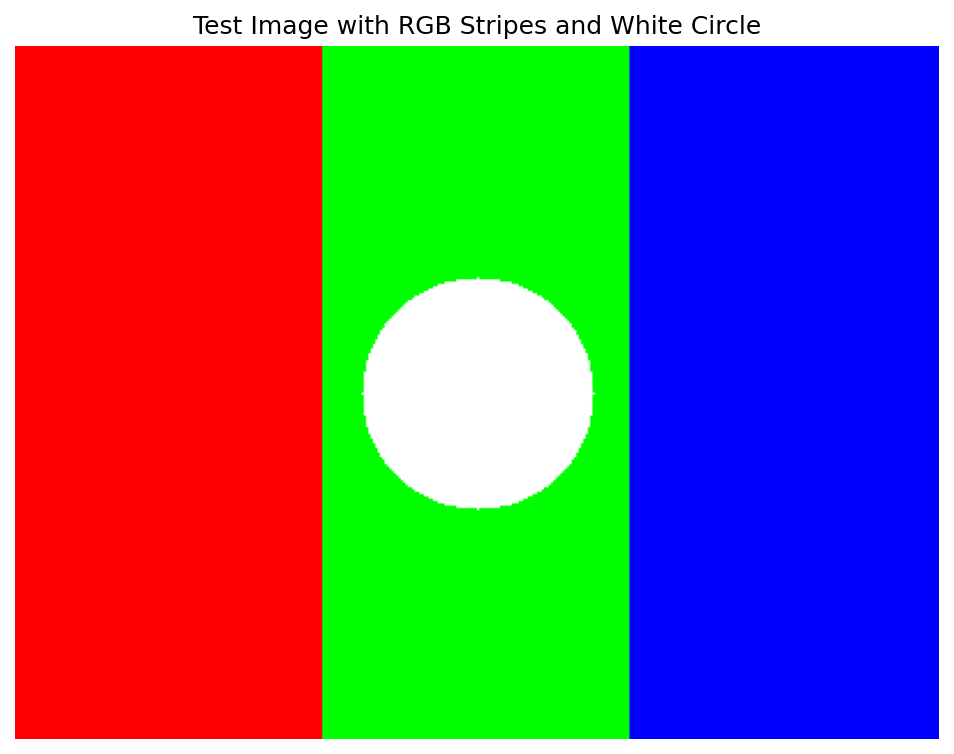
\includegraphics[width=\linewidth]{Figure/test_image.png}
        \caption{RGB}
    \end{subfigure}
    \caption{Gambar yang dihasilkan (sine\_wave\_test.png dan test\_image.png)}
    \label{fig:sine-rgb}
\end{figure}

\end{itemize}

\section{Bagian Laporan}

\subsection{Output Verifikasi Instalasi}
\textbf{Copy-paste output lengkap dari script \texttt{test\_multimedia.py} di sini:}

\begin{lstlisting}[caption=Output verifikasi instalasi]
[Generated 2s sine wave at 440Hz
Sample rate: 44100Hz
Total samples: 88200
Created test image: 400x300 pixels
Image shape: (300, 400, 3)
Image dtype: uint8]
\end{lstlisting}

\subsection{Screenshot Hasil Test}
\begin{itemize}
    \begin{figure}[H]
        \centering
        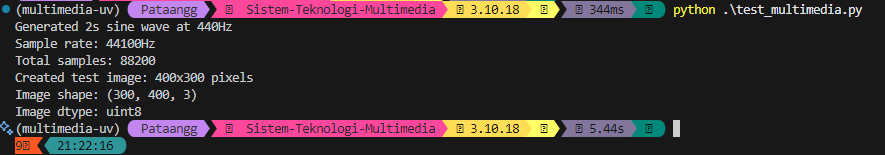
\includegraphics[width=0.8\textwidth]{Figure/img7.png}
        \caption{Screenshot output terminal dari kedua script}
        \vspace{0.1cm}
    \end{figure}
\end{itemize}

\subsection{Analisis dan Refleksi}
\textbf{Jawab pertanyaan berikut:}

\begin{enumerate}
    \item \textbf{Mengapa penting menggunakan environment terpisah untuk project multimedia?}
    
    \textit{Untuk \textbf{isolasi dependensi}. Supaya gaada konflik antar proyek yang membutuhkan versi library yang berbeda, memastikan \textbf{reproducibility} (proyek dapat dijalankan di mana saja dengan hasil yang sama), dan menjaga instalasi Python global tetap bersih}
    
    \item \textbf{Apa perbedaan utama antara conda, venv, dan uv? Mengapa Anda memilih tool yang Anda gunakan?}
    
    \textit{
    \begin{description}
        \item[\texttt{venv}] Bawaan Python, ringan, hanya mengelola paket Python
        \item[\texttt{conda}] Mengelola paket Python, versi Python, dan dependensi non-Python (misal: CUDA). Sangat kuat namun lebih lambat
        \item[\texttt{uv}] \textit{Installer} dan manajer \textit{environment} modern yang \textbf{sangat cepat} karena ditulis dalam Rust
    \end{description}
    \texttt{uv} dipilih karena \textbf{kecepatannya} yang superior dalam menginstal dan menyelesaikan dependensi, sangat menghemat waktu pada proyek dengan banyak library}
    
    \item \textbf{Library mana yang paling sulit diinstall dan mengapa?}
    
    \textit Gaada yang sulit sih semuanya bisa terinstall dengan baik
    
    \item \textbf{Bagaimana cara mengatasi masalah dependency conflict jika terjadi?}
    \textit{
    \begin{itemize}
        \item Baca pesan error untuk mengidentifikasi paket yang konflik
        \item Coba \textit{upgrade} paket utama yang menyebabkan masalah
        \item Tentukan versi paket yang kompatibel untuk semua dependensi secara manual
        \item Gunakan \textit{tool} manajemen seperti \texttt{poetry} buat lock versi library
        \item Kalo semua gagal, buat ulang \textit{environment} dari awal wkwkwk
    \end{itemize}
    }
    
    \item \textbf{Jelaskan fungsi dari masing-masing library yang berhasil Anda install!}
    \textit{
    \begin{itemize}
        \item \textbf{Audio Processing}
        \begin{itemize}
            \item \texttt{librosa}: Analisis dan ekstraksi fitur audio (spektogram, MFCC)
            \item \texttt{soundfile}: Membaca dan menulis berbagai format file audio
            \item \texttt{scipy}: Komputasi saintifik dan pemrosesan sinyal digital
        \end{itemize}
        \item \textbf{Image Processing}
        \begin{itemize}
            \item \texttt{opencv-python}: Pustaka utama untuk \textit{computer vision}
            \item \texttt{Pillow}: Manipulasi gambar dasar (crop, resize, rotasi)
            \item \texttt{scikit-image}: Algoritma analisis citra untuk riset
            \item \texttt{matplotlib}: Visualisasi data dan menampilkan gambar
        \end{itemize}
        \item \textbf{Video Processing}
        \begin{itemize}
            \item \texttt{moviepy}: Editing video melalui skrip (memotong, menggabung)
            \item \texttt{imageio-ffmpeg}: \textit{Wrapper} untuk FFmpeg agar bisa membaca/menulis format video
        \end{itemize}
        \item \textbf{General Purpose}
        \begin{itemize}
            \item \texttt{numpy}: Komputasi numerik fundamental dengan array N-dimensi
            \item \texttt{pandas}: Analisis dan manipulasi data terstruktur (tabel)
            \item \texttt{jupyter}: Lingkungan pemrograman interaktif (Notebook)
        \end{itemize}
    \end{itemize}
    }
\end{enumerate}

\subsection{Troubleshooting}
\textbf{Dokumentasikan masalah yang Anda hadapi (jika ada) dan cara mengatasinya:}

\begin{itemize}
    \item \textbf{Masalah 1:} \textit{["Which" command tidak dikenali]}
    \begin{figure}[H]
        \centering
        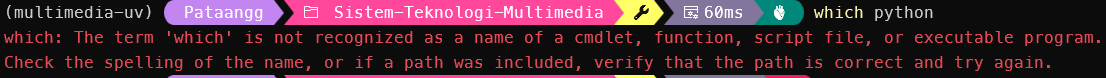
\includegraphics[width=0.8\textwidth]{Figure/img8.png}
        \caption{Which command invalid}
        \vspace{0.1cm}
    \end{figure}
    \textbf{Solusi:}
    \begin{itemize}
        \item Step 1. Tanya GPT-5
        \item Step 2. Ternyata masalahnya karena saya pake windows dan command "Which" itu cuma untuk MacOS dan Linux
        \item Step 3. Akhirnya saya coba command "where python" ternyata gabisa juga. Sebab command itu bisanya dipake di CMD sedangkan saya pakenya terminal (poweshell)

    \end{itemize}
\end{itemize}

\section{Export Environment untuk Reproduksi}
Sebagai langkah terakhir, export environment Anda agar dapat direproduksi:

\subsection{Untuk venv/uv}
\begin{lstlisting}[language=bash, caption=Export pip requirements]
pip freeze > requirements.txt
\end{lstlisting}

\textbf{Copy-paste isi file environment.yml atau requirements.txt di sini:}

\begin{lstlisting}[caption=Environment/Requirements file]
[anyio==4.10.0
argon2-cffi==25.1.0
argon2-cffi-bindings==25.1.0
arrow==1.3.0
asttokens==3.0.0
async-lru==2.0.5
attrs==25.3.0
audioread==3.0.1
babel==2.17.0
beautifulsoup4==4.13.5
bleach==6.2.0
certifi==2025.8.3
cffi==1.17.1
charset-normalizer==3.4.3
colorama==0.4.6
comm==0.2.3
contourpy==1.3.2
cycler==0.12.1
debugpy==1.8.16
decorator==5.2.1
defusedxml==0.7.1
exceptiongroup==1.3.0
executing==2.2.0
fastjsonschema==2.21.2
fonttools==4.59.1
fqdn==1.5.1
h11==0.16.0
httpcore==1.0.9
httpx==0.28.1
idna==3.10
imageio==2.37.0
imageio-ffmpeg==0.6.0
ipykernel==6.30.1
ipython==8.37.0
ipywidgets==8.1.7
isoduration==20.11.0
jedi==0.19.2
jinja2==3.1.6
joblib==1.5.1
json5==0.12.1
jsonpointer==3.0.0
jsonschema==4.25.1
jsonschema-specifications==2025.4.1
jupyter==1.1.1
jupyter-client==8.6.3
jupyter-console==6.6.3
jupyter-core==5.8.1
jupyter-events==0.12.0
jupyter-lsp==2.2.6
jupyter-server==2.17.0
jupyter-server-terminals==0.5.3
jupyterlab==4.4.6
jupyterlab-pygments==0.3.0
jupyterlab-server==2.27.3
jupyterlab-widgets==3.0.15
kiwisolver==1.4.9
lark==1.2.2
lazy-loader==0.4
librosa==0.11.0
llvmlite==0.44.0
markupsafe==3.0.2
matplotlib==3.10.5
matplotlib-inline==0.1.7
mistune==3.1.3
moviepy==2.2.1
msgpack==1.1.1
nbclient==0.10.2
nbconvert==7.16.6
nbformat==5.10.4
nest-asyncio==1.6.0
networkx==3.4.2
notebook==7.4.5
notebook-shim==0.2.4
numba==0.61.2
numpy==2.2.6
opencv-python==4.12.0.88
overrides==7.7.0
packaging==25.0
pandas==2.3.2
pandocfilters==1.5.1
parso==0.8.5
pillow==11.3.0
platformdirs==4.3.8
pooch==1.8.2
proglog==0.1.12
prometheus-client==0.22.1
prompt-toolkit==3.0.51
psutil==7.0.0
pure-eval==0.2.3
pycparser==2.22
pygments==2.19.2
pyparsing==3.2.3
python-dateutil==2.9.0.post0
python-dotenv==1.1.1
python-json-logger==3.3.0
pytz==2025.2
pywin32==311
pywinpty==3.0.0
pyyaml==6.0.2
pyzmq==27.0.2
referencing==0.36.2
requests==2.32.5
rfc3339-validator==0.1.4
rfc3986-validator==0.1.1
rfc3987-syntax==1.1.0
rpds-py==0.27.0
scikit-image==0.25.2
scikit-learn==1.7.1
scipy==1.15.3
send2trash==1.8.3
setuptools==80.9.0
six==1.17.0
sniffio==1.3.1
soundfile==0.13.1
soupsieve==2.7
soxr==0.5.0.post1
stack-data==0.6.3
terminado==0.18.1
threadpoolctl==3.6.0
tifffile==2025.5.10
tinycss2==1.4.0
tomli==2.2.1
tornado==6.5.2
tqdm==4.67.1
traitlets==5.14.3
types-python-dateutil==2.9.0.20250822
typing-extensions==4.15.0
tzdata==2025.2
uri-template==1.3.0
urllib3==2.5.0
wcwidth==0.2.13
webcolors==24.11.1
webencodings==0.5.1
websocket-client==1.8.0
widgetsnbextension==4.0.14
]
\end{lstlisting}

\section{Kesimpulan}
\textbf{Tuliskan kesimpulan Anda mengenai:}
\begin{itemize}
    \item Pengalaman setup Python environment untuk multimedia
    \item Persiapan untuk project multimedia selanjutnya
    \item Saran untuk mahasiswa lain yang akan melakukan setup serupa
\end{itemize}

\textit{
Setup environment Python buat multimedia itu wajib hukumnya biar nggak ribet sama konflik library. Makanya pakai \texttt{uv} atau \texttt{venv} itu bukan sekadar opsional, tapi memang keharusan. Dari pengalaman, \texttt{uv} kerasa banget cepetnya pas install paket gede kayak \texttt{OpenCV} dan \texttt{SciPy}}

\textbf{Biar aman ke depannya:}
\begin{enumerate}
    \item Selalu mulai dari environment baru yang bersih
    \item Habis install, langsung simpan \texttt{requirements.txt} pakai \texttt{uv pip freeze > requirements.txt}
    \item Pahami fungsi inti tiap library biar nggak salah pilih alat
\end{enumerate}

\textbf{Tips buat temen-temen lain:}
\begin{itemize}
    \item Jangan install global, bikin environment dari awal
    \item Lebih enak langsung pakai \texttt{uv}, simpel dan cepat
    \item Kalau error pas install, baca pesan error dulu—biasanya jelas apa yang kurang
    \item Install library seperlunya aja, biar gampang kalau ada masalah
\end{itemize}



\section{Referensi}
\begin{itemize}
    \item \href{https://docs.astral.sh/uv/}{UV Official Documentation}
    \item \href{https://chatgpt.com/share/68adcaac-f580-8006-bc89-1113529dff4d}{ChatGPT}
    \item \href{https://en.wikibooks.org/wiki/LaTeX}{LaTeX Wikibook: Comprehensive Guide}
    \item \href{https://www.overleaf.com/learn}{Overleaf Learn LaTeX Documentation}
\end{itemize}
\end{document}